\documentclass[floatfix,11pt]{revtex4}
%\documentclass[floatfix,11pt]{article}
\usepackage{color}
\usepackage{graphicx}
\usepackage{bm}
\usepackage{amsfonts}
\usepackage{mathrsfs}
\usepackage{amsmath}
\usepackage{amssymb}
\usepackage{setspace}
\usepackage{wrapfig}
\usepackage{fancyhdr}
\usepackage[labelfont=bf]{caption}
\usepackage{enumerate}
\usepackage{enumitem}
\usepackage{array}
\usepackage{natbib}
% \usepackage{pdfpages}
\newcolumntype{C}[1]{>{\centering\let\newline\\\arraybackslash\hspace{0pt}}m{#1}}

%----- Letter ----
\textwidth  = 6.5in
\textheight = 8.8in

\oddsidemargin = -0.in
\evensidemargin = 0.0in
\topmargin = -0.5in
\headheight = 0.5in
\headsep = 0.2in
\footskip = 0.4in

%%%%    HEADER     %%%%
\renewcommand{\headrulewidth}{0.75pt}
\pagestyle{fancyplain}
%\lhead{\small\textit{Mapping galaxies in spectral space}}
%\rhead{\small\textit{PI: Marina Meila}} 
\fancypagestyle{plain}

%%%%    FOOTER     %%%%
\renewcommand{\footrulewidth}{0.75pt}
\fancyfoot[LO]{\small\textit{DE-FOA-0002501}}
\fancyfoot[CO]{}
\fancyfoot[RO]{\small\textit{Page \thepage}}

%%%%%% my commands   %%%%%%


\newcommand{\dist}{{\rm dist}}
\newcommand{\epsi}{\varepsilon}
\newcommand{\D}{D}
\newcommand{\tily}{\tilde{y}}
\newcommand{\yg}{y_g}
\newcommand{\ygp}{y_{g'}}
\newcommand{\xg}{x_g}
\newcommand{\xgtrue}{x_{g}^{true}}
\newcommand{\xgptrue}{x_{g'}^{true}}
\newcommand{\xgf}{x_{g,l}}
\newcommand{\xgpf}{x_{g',l}}
\newcommand{\xgp}{x_{g'}}
\newcommand{\sigg}{\sigma_g}
\newcommand{\siggf}{\sigma_{g,l}}
\newcommand{\siggp}{\sigma_{g'}}
\newcommand{\siggpf}{\sigma_{g',l}}

\newcommand{\ml}{ML}
\newcommand{\sklearn}{{\tt scikit-learn}}
\newcommand{\mmani}{{\tt megaman}}
\newcommand{\gmani}{{\tt GigaMan}}

\newcommand{\comment}[1]{}
\newcommand{\mmp}[1]{\textcolor{blue}{MMP:#1}}
\newcommand{\bit}{\begin{itemize}}
\newcommand{\eit}{\end{itemize}}


\begin{document}
\begin{center}
{\sc Title} Vertical leap: Embedding high-dimensional data with functional analysis/consistency theorems and super-computers

\textbf{PI: Marina Meila} Professor of Statistics

University of Washington
% Department of Statistics, Box 354322, Seattle WA 98195-4322, 

Phone: 206-543-8484,  {\tt mmp@stat.washington.edu}

{\textbf DE-FOA-0002501}

\line(1,0){480}
\end{center}
\singlespacing
\vspace{-.75cm}
\noindent\begin{tabular}{lll}
\multicolumn{3}{c}{Examples of data reduction by low dimensional embedding and smoothing}\\
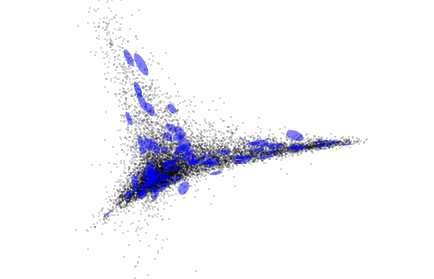
\includegraphics[width=2.1in]{Figures/word2vec_rmetric_plot_noaxis_trim.png} &
%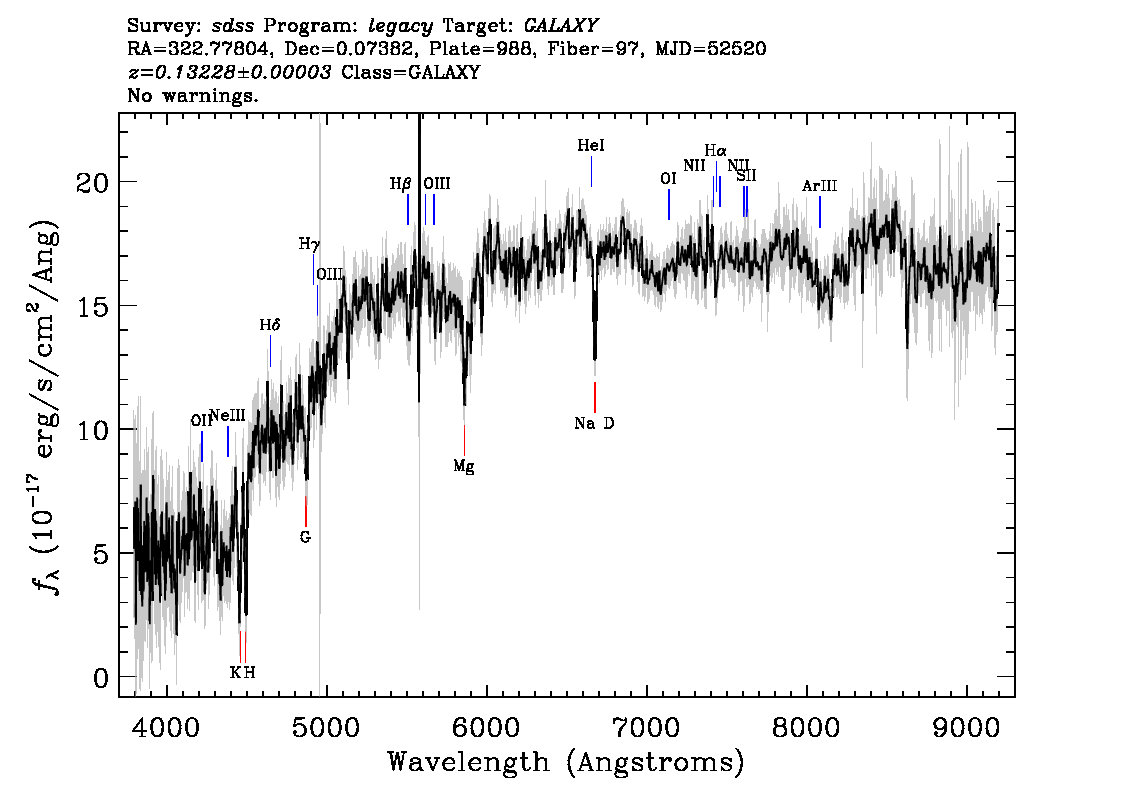
\includegraphics[width=2.2in]{Figures/specById_asp.png} & 
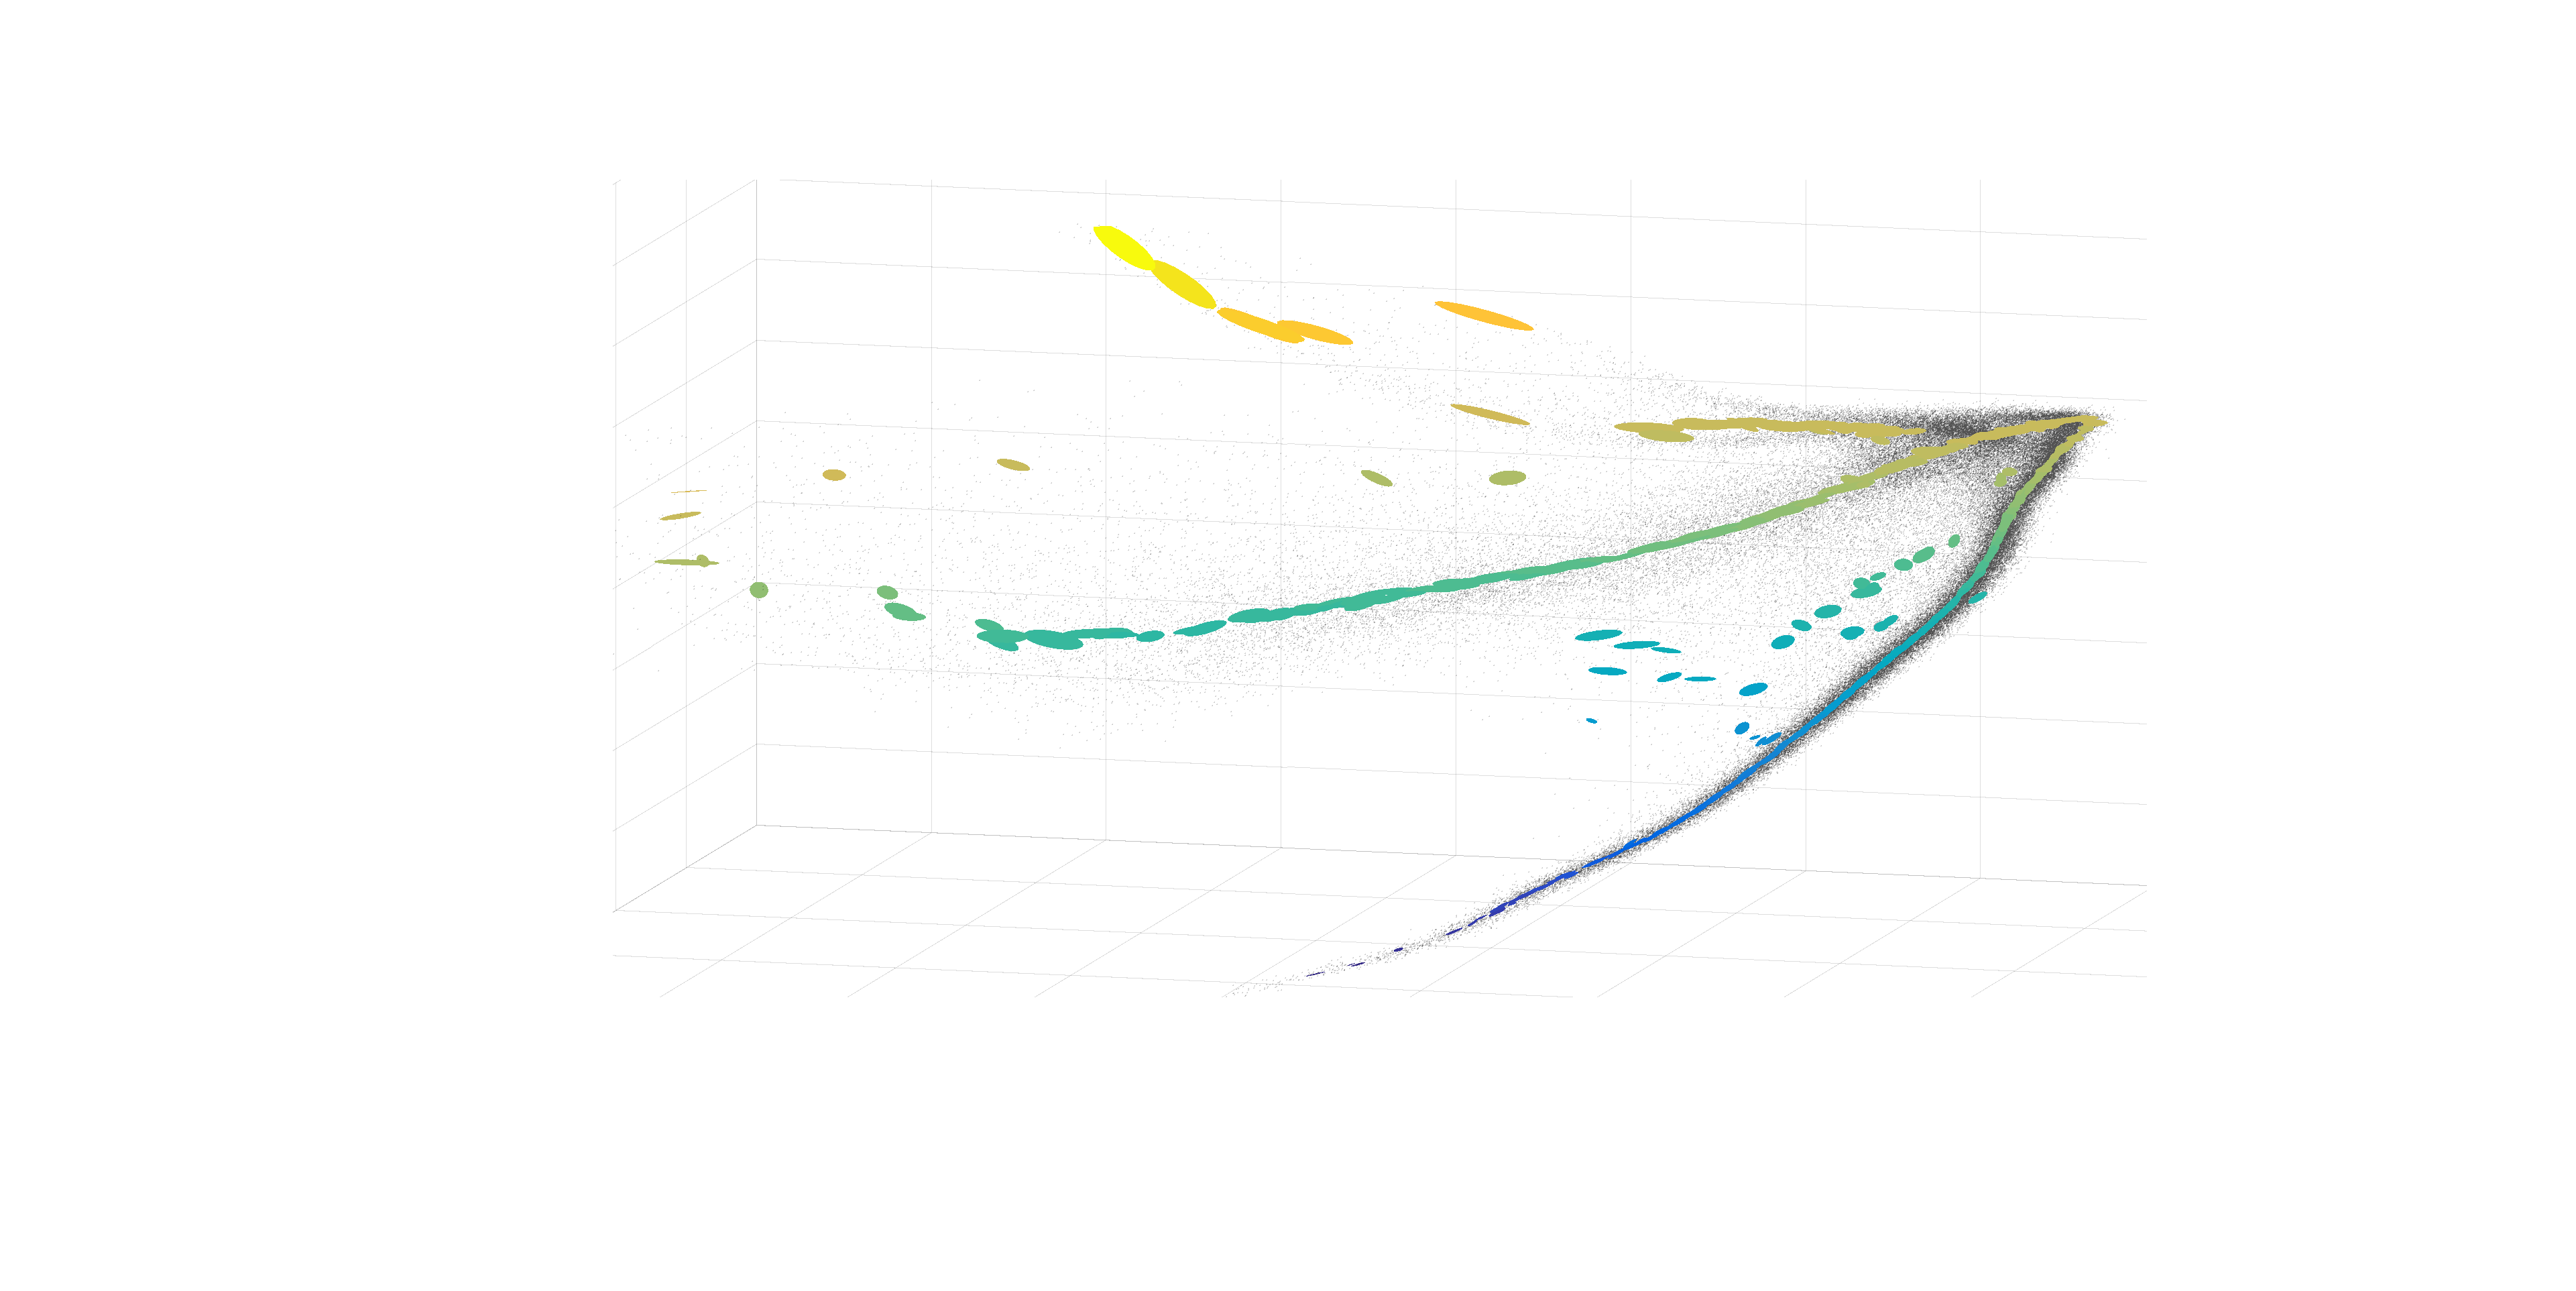
\includegraphics[width=2.5in,clip=]{Figures/spectrum_data_before-trim.pdf} 
&
\includegraphics[width=2.5in,clip=]{Figures/smoothed_velocity_field_alpha_50.pdf}\\
\multicolumn{2}{l}{
\parbox[t]{4.5in}{{\bf Left:} 3D embedding of 3,000,000 words and phrases represented in 300 dimensions from {\tt https://code.google.com/archive/p/word2vec/}; {\bf middle:} 3D embedding of 665,000 spectra of galaxies from {\tt www.sdss.org} with 3750 wavelengths}}
&
\parbox{2.5in}{{\bf right:} Smoothed velocity field of 20,000 ocean buoys from {\tt https://www.ndbc.noaa.gov}}
\\
\end{tabular}
\begin{tabular}{llll}
\multicolumn{3}{c}{Naive embeddings introduce artefacts}
&
Measuring embedding distortion
\\
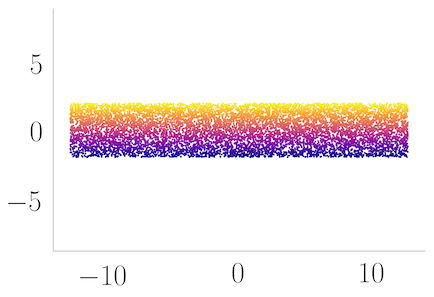
\includegraphics[width=1.7in]{Figures/D1_original_data.png} &
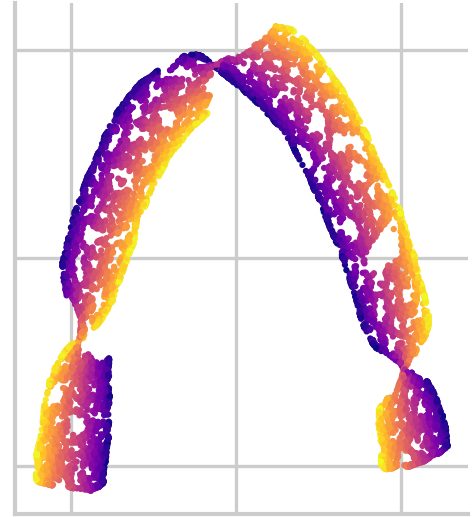
\includegraphics[width=0.8in]{Figures/umap_mindist_comp.png} &
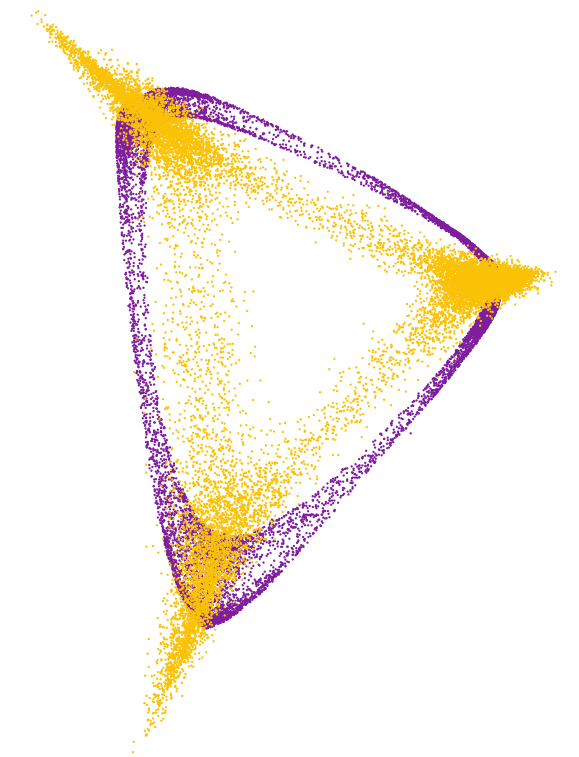
\includegraphics[width=1.2in,angle=90]{Figures/geometric_vs_normalized.png}
&
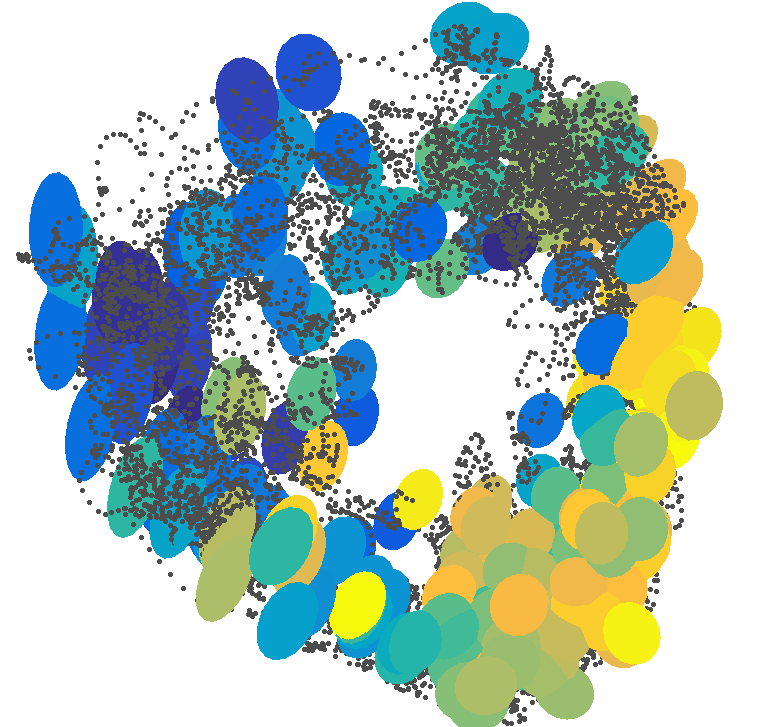
\includegraphics[width=1.2in]{Figures/aspirin-postclu1-phi234Rmetric-tau22.png}
\\
\multicolumn{3}{l}{\parbox{4.7in}{{\bf Left:} Embedding of a 2D strip by UMAP, showing 4 clusters inexistent in the original data; {\bf middle:} two embeddings of molecular configurations of ethanol; the original data is a torus.}}\\
\end{tabular}

What is proposed: \gmani, a non-linear dimension reduction toolbox
in python, that scales to data matrices of order $n\times p \sim
10^{12}$, which implements the state of the art in the mathematics and
statistics of high dimensional geometric learning.

\textbf{Motivation} We are concerned with data in the form of
high-dimensional ``point clouds'', such as spectra of galaxies (with
dimension given by the number of spectral wavelengths), spatial
locations of the atoms in a molecule (with dimension given by the number atoms $\times$ spatial dimension 2 or 3), state space of a dynamical system. Non-vector data for which a {\em distance} between points can
be calculated, such as biological sequences, words and phrases, job
descriptions, images, can also be considered point cloud data. 

Often times, the physical processes generating/underlying these observations have fewer degrees of freedom than the data dimension, and they can be described by mathematically by manifolds and vector fields thereon.  Significant data reduction can be achieved by non-linear dimension reduction mehods, since a very large number of high dimensional data are described by a much smaller number of degrees of freedom (for example, while image resolution can grow from Mega-pixels into Giga-, the image contens does not become richer at the same rate). This class of methods is known as {\em (non-linear) embedding} methods. 

\mmp{Too much probably:} Embeddings know-how is relevant other data reduction in approaches too. One is smoothing the data, by projecting it onto a local manifold; the other is subsampling the regions where the data is too dense, and summarizing the local geometry by means of indexing, meta-information, or core-sets.

Data reduction for the sciences must come with guarantees of
  reproducibility (e.g. outputs not sensitive to initialization of
  algorithm), stability (outputs not sensitive to variations in
  sample), as well as with rigurous methods to quantify the loss of
  information and the variability of the result, and with
  guarantees of preserving desired properties/features/(geometric)
  characteristics

\textbf{Challenges} Estimating non-linear geometry from point cloud data is very hard statistically and mathematically. Because of the non-linearity of the space, e.g.  (variable) local curvature, naive methods of dimension reduction are generally biased, introducing distortions, or even inconsistent, tending to unreasonable/degenerate limits when $n\rightarrow \infty$. ``Errors don't average to 0'' in non-linear geometric estimation. The statistical and mathematical methods needed to analyze the properties of embedding algorithms and to design consistent, unbiased, ones are highly technical, and are a field under development. [Proof that of the most popular methods LLE, t-SNE, UMAP are unstable and inconsistent in the limit, depend on parameters that must be set by eyeballing]

However, these results are too technical to be read by most scientists, engineers and computer scientists. Moreover, the results depend on unspecified constants and on properties of the data. To bring them to be relevant to science one must develop methods to measure and test if the theoretical conditions hold for the data at hand. One must also select those theoretical results that relie on testable assumptions, and that best fit the statistical structure of the problem. For example, the embedding algorithms must adapt to  the density of molecular configurations in state space can vary exponentially, or to the variation of measurements noise with red-shift and wavelength in spectrographic observations of galaxies, and exploit these properties, whenever possible.

This is a barrier to the adoption of the state of the art knowledge. 

\bit
\item Embedding algorithms relie on a form of interpolation between neighbors (are similar to kernel density estimation). Finding neighbors in high dimensions and large data sets is the main computational bottleneck. 
\item Eigendecompositions is the {\em perceived} bottleneck, but the PI's own experience and communications with experts show that with careful/expert reweighing, preprocessing, the eigendecomposition step is more tractable than the nearest neighbor step. In particular, eigendecomposition does not depend on the data dimension $p$, but only on the sample size $n$. 
\item Even if phenomena well approximated by manifolds, in fact they are multiscale (or equivalently, noise has structure, is not i.i.d. and not isotropic), and rarely is the dimension constant. One of the contributions of this proposal is to rigurously develop embedding methods with variable dimension (unions of manifold, stratified spaces)
\item What if data can't be stored in memory? Distributed data? I'd rather not deal with it now. We'll see. 
  \eit

What we will do, again.
\bit
\item  {\em Methods} for nearest neighbor search, data indexing and subsampling, suitable for non-linear embedding. The methods will be grounded in state of the art statistical theory. Main contribution under this grant: original research on how to measure/test from data when theoretical conditions apply; to choose the optimal embedding method for a particular data, to derive what guarantees can be obtained from theory for the reduction of a real data set. 
\item {\em Software distribution} Release of a suite of python packages implementing the above methods, and specializing them for \mmp{fill in specific tasks} in \mmp{astrononomy, chemistry} 
\eit

  
  {\bf Why non-lin dim reduction great for scientific data}
  \bit
  \item Often data
dimension is a function of the resolution of the instrument and does
only slowly add new degrees of freedom. Hence, higher $p$ means
sharper measurements, less instrument noise: good. Highly non-uniform
sampling (e.g. molecular configurations are subject to Boltzmann
distribution, with exponential variations of density). When data
non-uniform, in highly concentrated regions it becomes redundant --
only a freaction of it is sufficient to estimate the geometry;
statistically, subsampling the data in this regime produces a faster
converging embedding.

\item Nearest-neighbor methods have been proved to be {\em adaptive} to intrinsic dimension.
\item Good statistics implies stable and efficient computation. In particular, complexity of geometric algorithms, if properly tuned, depends on the {\em intrinsic dimension/number of free parameters}, not on data dimension (with the exception of distance computations). 
\item The most theoretically efficient algorithms do not become so until data isvery large.
\eit

{\bf What we will do}\footnote{The number of M's after a task is the amount of original statistical/algorithm/methodology research needed to produce an implementable method}
\bit
\item Design implementable algorithm for approximate fast nearest neighbor method based on theoretical state of the art. Main sources Indyk, Charikar, Razenshteyn. MM
\item Proof that {\em this} approximate nearest neighbor is sufficient to assure convergence when used with manifold learning algorithms Source: Fefferman et collabs\footnote{Fefferman is Fields medalist.} MMM
\item The methods above depend on constants with undknown values. Design methods to estimate the constants from data (e.g. a form of CV, by geometric consistency, etc). MMM
\item Summarizing/subsampling big data: Coresets and hierachical indexing. Sources TBW. M 
\item Translate the methods above into algorithms. M
\item Implement the algorithms efficiently to obtain a toolbox of neighborhood construction algorithms, and a toolbox of embedding algorithms. These will be called the core algorithms. M
\item Develop around the core algorithms a suite of other methods.
 \bit
 \item Preprocessing: subsampling, estimating the local neighborhood size, estimating the intrinsic dimension, data indexing (related to subsampling) M
 \item Non-embedding methods based on neighborhood graphs: L1 Laplacian and Helmholtz-Hodge decomposition, other TDA applications, kernel regression on manifolds M
 \item Postprocessing: estimating/correcting the embedding by metric learning and Riemannian Relaxation, estimating the noise (e.g. MSE, locally), stratifying the data by dimension, MM
   \eit
 \item Data reduction for chemistry and materials sciences
 \item Data reduction for astronomy 
   \bit
 \item LSST
 \item simulated data
   \eit
 \eit


\underline{\bf Team expertise} Team of exceptional depth and breadth.
MMP has spent more than 10 years pondering the problems in non-parametric data analysis and geometric learning. She is aware of of the theoretical advances, and capable to discern their significance w.r.t. practical problems and existing data. More specifically, theorems must relie on testable assumptions to be of methodological value. The PI's contribution is focused on this aspect: how to make mathematics meet real life problems? What can we measure from real data so that we can guarantee that theory applies?
The PI is an expert in Machine Learning, and has a long track record of developing algorithms in geometric data analysis and unsupervised learning, and of deploying them as software packages.

All team members are long term collaborators, and all are Senior Fellows of the eSCience Institute. Meila, Connolly and Ivezic collaborated on more than five grant proposals; Meila and Beck collaborated on four grant proposals, two of them funded by the DE under FOA .... Meila and Vasquez-Mayagoitia collaborated on the ALCF Grant .... As part of this collaboration, the software \mmani~was ported on the Theta, and UW student Yu-chia Chen visited ALCF. \mmani~originated in the first Data Science Incubator as a collaboration between Meila and Jake VanderPlas. 
Dr. Marina Meila is Professor of Statistics with adjunct appointments in Computer Science and Electrical Engineering at UW. Her primary expertise is in machine learning, specifically in statistical learning, high-dimensional inference and big data. She has widely recognized contributions to learning in graphical models, spectral clustering,37 non-linear dimension reduction,38 Bayesian statistics,39 and sparse estimation. Her group developed the open source Python package “megaman”40 (over 45K downloads) which performs dimension reduction and other ML tasks on millions of points in thousands of dimensions. She has authored 108 publications and has an h-index of 36.
Dr. David Beck is the Director of Research for the eScience Institute, the University of Washington’s central institute for data science and machine learning. He directs a team that develops new data science methods and software in coordination with researchers across the pacific northwest. He is an expert in the development and application of open source tools for data science and machine learning in areas such as energy, environment, and health. He is the author over 80 peer reviewed publications with a h-index of 31.
%The PI is in the unique position to be aware of the theoretical advances in manifold learning and geometric data analysis, 


%brings extensive experience in ML, from the statistical issues \cite{PerraultMMcQueen:nips17} to software \cite{mcqueenMVdpZ:megaman16,*mcqueenMVdpZ:megaman-jmlr16}


{\bf Previous work}

{\bf Existing support} No other funding exists for this project. collaborative grant of 170M CPU hours at the Argonne Labs Computing Facility (see CV) since September 2017 for the PI's research on manifold learning in chemistry.

{\bf Readiness} The package {\tt megaman}\footnote{{\tt http://mmp2.github.io/megaman}} \cite{mcqueenMVdpZ:megaman16,*mcqueenMVdpZ:megaman-jmlr16} implements all the manifold learning algorithms described in this proposal. Our pilot experiments (one shown in Fig. 3) and \cite{Yip04} \comment{prove that that we have the computing resources and }strongly suggest that low dimensional structure exists in the SDSS data. The PI and co-PI are co-mentoring PhD student Yu-chia Chen, and are committed to developing open source machine learning software (e.g {\tt megaman}, contributions to {\tt scikit-learn}). \comment{With infrastructure and collaboration in place, we}We request funding for one graduate student, and one undergraduate student (only computing costs) for 12 months.



\vspace{-2.1em}
\bibliographystyle{abbrv}
\bibliography{proposal,SDSS_LLE}

\vspace{0.6em}

\vspace{0.6em}

\newpage
\centerline{\textbf{Senior Personnel}}
\begin{tabular}{llll}
  Last name & First name & Title & Institution\\
  \hline
Meila & Marina & Professor & University of Washington\\
Beck & David & Professor &  University of Washington\\
Ivezic & Zeljko & Professor &  University of Washington \\
Connolly & Andrew & Professor &  University of Washington (???)\\
Juric & Mario & Associate Professor &  University of Washington (???)\\
Vasquez-Mayagoitia & Alvaro & Computational Scientist & Argonne National Computing Facility\\
\end{tabular}

\vspace{0.4em}
\centering{\textbf{Collaborators, Co-editors, and Graduate and Postdoctoral Advisors and Advisees of the PI and Senior/Key Personnel}}
\begin{tabular}{llll}

\end{tabular}

\end{document}
